\documentclass[12pt, a4paper]{article}

\usepackage[margin=2.5cm]{geometry} 
\usepackage{fancyhdr}               
\usepackage{hyperref}               
\usepackage{graphicx}               
\usepackage{float}                  
\usepackage{titlesec}
\usepackage{wrapfig}         
\usepackage{subcaption}

% Pengaturan Header dan Footer
\pagestyle{fancy}
\fancyhf{}
\lhead{\textbf{Nama:} Khalilullah Al Faath}   
\rhead{\textbf{NIM:} 25/566643/PPA/07139}        
\renewcommand{\headrulewidth}{0.4pt}         
\renewcommand{\footrulewidth}{0.4pt}         


\begin{document}

\begin{center}
    \large \textbf{Laporan Assignment 1 \\ Comparing Ranked Retrieval Models} \\[0.2cm]
    \large Sistem Temu Balik Informasi  \\[0.5cm]
\end{center}


\section{Pranala Kode}
Hasil \textit{running} implementasi kode dapat diakses di pranala repositori GitHub berikut \url{https://github.com/khalilullahalfaath/comparing-ranked-retrieval-models/blob/main/1_STBI.ipynb}.

\section{Deskripsi dan Karakteristik Data}
Dataset yang digunakan terdiri dari korpus berita berbahasa Indonesia dengan total 14.334 dokumen. Berdasarkan hasil eksplorasi data, korpus ini memiliki total kata sebanyak 5.524.047 kata, dengan rata-rata panjang dokumen sekitar 385 kata per berita. Gambar!\ref{fig:distribusi} Sesuai dengan spesifikasi tugas, tidak ada proses \textit{pre-processing} yang dilakukan.

\begin{figure}[h]
    \centering
    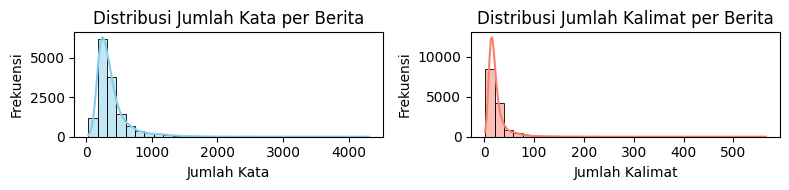
\includegraphics[width=1\textwidth]{distribusi.png}
    \caption{Distribusi jumlah kata dan kalimat pada setiap dokumen kebanyakannya berjumlah 300-an dengan jumlah kalimat kurang dari 20.}
    \label{fig:distribusi}
\end{figure}

\section{Analisis Waktu Komputasi (\textit{Indexing})}
Proses pembangunan matriks representasi dokumen (\textit{indexing}) menunjukkan perbedaan waktu komputasi yang sangat signifikan di antara ketiga model:
\begin{itemize}
    \item \textbf{TF-IDF (4,29 detik):} Merupakan model tercepat karena hanya melakukan ekstraksi fitur berbasis frekuensi statistik dan membentuk \textit{sparse matrix} berdimensi (14334, 90903).
    \item \textbf{Word2Vec (13,42 detik):} Memanfaatkan pre-trained model yang didapatkan dari \url{https://www.kaggle.com/datasets/bhimantoros/pretrained-word2vec-indonesia} dan menghasilkan w2v matrix dengan ukuran (14334, 400).
    \item \textbf{IndoBERT (385,24 detik):} Memanfaatkan pre-trained model yang didapatkan dari \url{https://huggingface.co/indobenchmark/indobert-base-p1} dan menghasilkan $bert\_matrix$ berdimensi (14334, 768).
\end{itemize}

\section{Evaluasi Kualitatif}
Pengujian menggunakan 10 kueri skenario mengungkap kelebihan dan kelemahan masing-masing model terhadap data mentah:
\begin{enumerate}
    \item TODO
\end{enumerate}

\section{Analisis Waktu Pencarian (\textit{Query Time})}
Metrik evaluasi waktu pencarian (\textit{Cosine Similarity}) pada Top-3 dokumen menghasilkan urutan rata-rata: \textbf{Word2Vec (0,029 detik) $<$ IndoBERT (0,086 detik) $<$ TF-IDF (0,093 detik)}.
Word2Vec mendominasi kecepatan pencarian karena hanya mengukur jarak antar vektor pada matriks padat berdimensi rendah (400). Sebaliknya, meskipun proses \textit{indexing} TF-IDF sangat cepat, kalkulasi kosinus pada saat pencarian sedikit terhambat oleh besarnya ukuran ruang fitur \textit{sparse matrix} (lebih dari 90 ribu kosakata).

\end{document}